%
% This is the LaTeX template file for lecture notes for EE 382C/EE 361C.
%
% To familiarize yourself with this template, the body contains
% some examples of its use.  Look them over.  Then you can
% run LaTeX on this file.  After you have LaTeXed this file then
% you can look over the result either by printing it out with
% dvips or using xdvi.
%
% This template is based on the template for Prof. Sinclair's CS 270.

\documentclass[twoside]{article}
\usepackage{graphics}
\usepackage{tikz}
\usepackage{pgfplots}
\pgfplotsset{compat=1.15}
\usetikzlibrary{intersections}
\usetikzlibrary{patterns}
\setlength{\oddsidemargin}{0.25 in}
\setlength{\evensidemargin}{-0.25 in}
\setlength{\topmargin}{-0.6 in}
\setlength{\textwidth}{6.5 in}
\setlength{\textheight}{8.5 in}
\setlength{\headsep}{0.75 in}
\setlength{\parindent}{0 in}
\setlength{\parskip}{0.1 in}

%
% The following commands set up the lecnum (lecture number)
% counter and make various numbering schemes work relative
% to the lecture number.
%
\newcounter{lecnum}
\renewcommand{\thepage}{\thelecnum-\arabic{page}}
\renewcommand{\thesection}{\thelecnum.\arabic{section}}
\renewcommand{\theequation}{\thelecnum.\arabic{equation}}
\renewcommand{\thefigure}{\thelecnum.\arabic{figure}}
\renewcommand{\thetable}{\thelecnum.\arabic{table}}

%
% The following macro is used to generate the header.
%
\newcommand{\drawle}{-- (rel axis cs:1,1) -- (rel axis cs:1,0) -- (rel axis cs:0,0) \closedcycle}

\newcommand{\lecture}[4]{
   \pagestyle{myheadings}
   \thispagestyle{plain}
   \newpage
   \setcounter{lecnum}{#1}
   \setcounter{page}{1}
   \noindent
   \begin{center}
   \framebox{
      \vbox{\vspace{2mm}
    \hbox to 6.28in { {\bf EE 382V: Social Computing
                        \hfill Fall 2018} }
       \vspace{4mm}
       \hbox to 6.28in { {\Large \hfill Homework 2: #2  \hfill} }
       \vspace{2mm}
       \hbox to 6.28in { {\it Partner1: #3 \hfill Partner2: #4} }
      \vspace{2mm}}
   }
   \end{center}
   \markboth{EE382V:Social Computing HW2: #2}{EE382V:Social Computing HW2: #2}
   %{\bf Disclaimer}: {\it These notes have not been subjected to the
   %usual scrutiny reserved for formal publications.  They may be distributed
   %outside this class only with the permission of the Instructor.}
   \vspace*{4mm}
}

%
% Convention for citations is authors' initials followed by the year.
% For example, to cite a paper by Leighton and Maggs you would type
% \cite{LM89}, and to cite a paper by Strassen you would type \cite{S69}.
% (To avoid bibliography problems, for now we redefine the \cite command.)
% Also commands that create a suitable format for the reference list.
\renewcommand{\cite}[1]{[#1]}
\def\beginrefs{\begin{list}%
        {[\arabic{equation}]}{\usecounter{equation}
         \setlength{\leftmargin}{2.0truecm}\setlength{\labelsep}{0.4truecm}%
         \setlength{\labelwidth}{1.6truecm}}}
\def\endrefs{\end{list}}
\def\bibentry#1{\item[\hbox{[#1]}]}

%Use this command for a figure; it puts a figure in wherever you want it.
%usage: \fig{NUMBER}{SPACE-IN-INCHES}{CAPTION}
\newcommand{\fig}[3]{
			\vspace{#2}
			\begin{center}
			Figure \thelecnum.#1:~#3
			\end{center}
	}
% Use these for theorems, lemmas, proofs, etc.
\newtheorem{theorem}{Theorem}[lecnum]
\newtheorem{lemma}[theorem]{Lemma}
\newtheorem{proposition}[theorem]{Proposition}
\newtheorem{claim}[theorem]{Claim}
\newtheorem{corollary}[theorem]{Corollary}
\newtheorem{definition}[theorem]{Definition}
\newenvironment{proof}{{\bf Proof:}}{\hfill\rule{2mm}{2mm}}

% **** IF YOU WANT TO DEFINE ADDITIONAL MACROS FOR YOURSELF, PUT THEM HERE:

\begin{document}
%FILL IN THE RIGHT INFO.
%\lecture{**LECTURE-NUMBER**}{**DATE**}{**LECTURER**}{**SCRIBE**}
\lecture{1}{October 21}{Javier Palomares}{Porter Perry}
%\footnotetext{These notes are partially based on those of Nigel Mansell.}

% **** YOUR NOTES GO HERE:

% Some general latex examples and examples making use of the
% macros follow.  
%**** IN GENERAL, BE BRIEF. LONG SCRIBE NOTES, NO MATTER HOW WELL WRITTEN,
%**** ARE NEVER READ BY ANYBODY.
\section{Question 1}
Consider the following linear program.

max $2x_{1} + 6x_{2}$\\
subject to\\
$4x_{1} + x_{2} \leq 8$,\\
$x_{1} + 2x_{2} \leq 6$,\\
$x_{1}, x_{2} \geq 0$,\\

(a) Draw the feasible solution space on $x_{1}$,$x_{2}$ plane.\\
(b) Give all the vertices of the feasible solution space.\\
(c) What is the optimal value of the objective function?\\
(d) Give the dual of the above primal problem.\\
(e) Draw the feasible solution space for the dual version.\\
(f) What is the optimal solution of the dual version of the problem?

\subsection{Answer 1a}

%\iffalse
\begin{tikzpicture}
    \begin{axis}[
        axis on top, smooth,
        axis line style=very thick,
        axis x line=bottom,
        axis y line=left,
        ymin=-1,ymax=7,xmin=-1,xmax=7,
        xlabel=$x_1$, ylabel=$x_2$,grid=major
        ]
        \addplot[
            name path global=firstline,
            very thick, 
            domain=-10:10
            ]
            coordinates {(0,-10) (0,10)};
        \addplot[
            name path global=secondline,
            very thick, 
            domain=-10:10
            ]
            {3 - 0.5*x};
        \addplot[
            name path global=thirdline,
            very thick, 
            domain=-10:10
            ]
            {8 - 4*x};
        \addplot[
            name path global=fourthline,
            very thick, 
            domain=-10:10
            ] 
            coordinates {(-10,0) (10,0)};
        \fill[
        name intersections={of=firstline and secondline,by=point1},
        name intersections={of=secondline and thirdline,by=point2},
        name intersections={of=thirdline and fourthline,by=point3},
        name intersections={of=fourthline and firstline,by=point4},
        ]
        [very thick,
        draw=orange,
        pattern=crosshatch dots,
        pattern color=green!60!white
        ]
        (point1)--(point2)--(point3)--(point4)--(point1);
    \end{axis}
\end{tikzpicture}
%\fi

\subsection{Answer 1b}

Feasible region corner vertices: \\
$(0, 0)$ \\
$(0, 3)$ \\
$(10/7, 16/7)$ \\
$(2, 0)$ 

\subsection{Answer 1c}

The optimal value of the Primal objective function is 18.

\subsection{Answer 1d}

Dual Problem: \\

min $8y_{1} + 6y_{2}$\\
subject to\\
$4y_{1} + y_{2} \geq 2$,\\
$y_{1} + 2y_{2} \geq 6$,\\
$y_{1}, y_{2} \geq 0$,\\

\subsection{Answer 1e}

%\iffalse
\begin{tikzpicture}
    \begin{axis}[
        axis on top, smooth,
        axis line style=very thick,
        axis x line=bottom,
        axis y line=left,
        ymin=-1,ymax=7,xmin=-1,xmax=7,
        xlabel=$y_1$, ylabel=$y_2$,grid=major
        ]
        \addplot[
            name path global=firstline,
            very thick, 
            domain=-10:10
            ]
            {2 - 4*x};
        \addplot[
            name path global=secondline,
            very thick, 
            domain=-10:10
            ]
            coordinates {(0,-10) (0,10)}; %vertical line representing x=0
        \addplot[
            name path global=thirdline,
            very thick, 
            domain=-10:10
            ]
            {3 - 0.5*x};
        \addplot[
            name path global=fourthline,
            very thick, 
            domain=-10:10
            ] 
            coordinates {(-10,0) (10,0)}; %horizontal line representing y=0
        \addplot[
            name path global=fifthline,
            very thick, 
            domain=-10:10
            ] 
            coordinates {(10,-10) (10,10)}; %vertical line representing x=10
        \addplot[
            name path global=sixthline,
            very thick, 
            domain=-10:10
            ] 
            coordinates {(-10,10) (10,10)}; %horizontal line representing y=10
        \fill[
        name intersections={of=secondline and thirdline,by=point2},
        name intersections={of=thirdline and fourthline,by=point3},
        name intersections={of=fourthline and fifthline,by=point4},
        name intersections={of=fifthline and sixthline,by=point5},
        name intersections={of=sixthline and secondline,by=point6},
        ]
        [very thick,
        draw=orange,
        pattern=crosshatch dots,
        pattern color=green!60!white
        ]
        (point2)--(point3)--(point4)--(point5)--(point6)--(point2);
    \end{axis}
\end{tikzpicture}
%\fi

\subsection{Answer 1f}

The optimum solution for the Dual objective function is $(y_{1}, y_{2}) = (0, 3)$, which gives an optimum value of 18 (same as for the primal).

\section{Question 2}
Show that the man-oriented Gale-Shapley algorithm gives the woman-pessimal stable matching, i.e., each woman is paired with her worst valid partner of all stable matchings. 

\subsection{Answer 2}

\textbf{Proof} by contradiction:

Let $M = \{ \ldots, (m, w), \ldots \}$ be the set male optimal marriages from the output of the male-oriented Gale-Shapley algorithm. 

Suppose that there exists a stable that is not woman pessimal, represented by $M' = \{ \ldots, (m', w), \ldots, (m, w'), \ldots\}$ such that $m$ is not the pessimal choice for $w$. In this scenario , $w$ prefers $m$ over $m'$. However, if the stable marriage is also male optimal, then $m$ prefers $w$ over $w'$. 

The above case is a contradiction because this creates a blocking pair, which proves that such a marriage $M'$ is not stable. Therefore, a male optimal pairing must be woman pessimal.

\section{Question 3}
Suppose that you are given an instance of a stable marriage problem, i.e., the ordered lists of men preferences and the ordered list of women preferences.\\

(a) You are given a particular couple $(m, w)$ as an additional input. Give an algorithm to determine if there exists a stable marriage with $m$ assigned to $w$.\\
(b) What certificate can you give to your friend to show that there is no stable marriage with $(m, w)$ pair?\\
(c) What certificate can you give to your friend to show that there is a stable marriage with ($m, w$) pair?

\subsection{Answer 3a}

Modify the Gale-Shapely stable marriage algorithm with a constraint that the $(m*,w*)$ is already assigned (married).

\textbf{Inputs}:\\
1. $mPref$: data structure containing preferences for each man \\
2. $wPref$: data structure containing preferences for each woman \\
3. $mrank$: where $mrank[i][j]$ indicates the rank of woman $j$ for man $i$; higher preference correlates to lower rank \\
4. $wrank$: where $wrank[i][j]$ indicates the rank of man $j$ for woman $i$; higher preference correlates to lower rank \\

\textbf{Algorithm}:\\
1. freelist = list of men who are free (initially has all men except $m*$) \\
2. while (freelist is not empty): \\
\hspace*{7mm} 3. choose some man $m$ from freelist \\
\hspace*{7mm} 4. $m$ proposes to his most preferred woman $w$ that he has not already proposed to, and is not $w*$ \\
\hspace*{7mm} 5. if $w$ is free: \\
\hspace*{14mm} 6. $w$ accepts proposal (assign $m$ to $w$) \\ 
\hspace*{7mm} 7. else: // $w$ is already engaged to $m′$ \\
\hspace*{14mm} 8. if $wrank[w][m] > wrank[w][m′]$: // $w$ prefers $m′$ \\
\hspace*{21mm} 9. add $m$ back to freelist // reject $m$; $w$ still engaged to $m′$ \\
\hspace*{14mm} 10. else: \\
\hspace*{21mm} 11. add $m′$ back to the freelist // reject $m′$ \\ 
\hspace*{21mm} 12. $w$ gets engaged to $m$ \\
13. for each $(m, w)$ marriage assignment that isnot $(m*, w*)$ \\
\hspace*{14mm} 14. if $mrank[m][w] > mrank[m][w*]$ and $wrank[w*][m*] > wrank[w*][m]$: \\
\hspace*{21mm} 15. Print blocking pair found, then exit \\
\hspace*{14mm} 16. else: \\
\hspace*{21mm} 17. Continue through for loop to next marriage assignment \\ 
18. Print stable marriage exists with $m*$ assigned to $w*$

\subsection{Answer 3b}

The certificate that can be shown to prove that their is no stable marriage with the ($m, w$) pair is to show that their exists a blocking pair, which is couple pairing ($m', w'$) in which  $m$ prefers $w'$ to $w$, and $w'$ prefers $m$ to $m'$.  

\subsection{Answer 3c}



\end{document}





